% Chapter 4

% variables
\newcommand{\pdirfour}{chapters/plots/chapter4}

\chapter{Results}

\label{chapter4}

The analysis strategy, background sources, selection criteria, and computed signal yield was described in the previous chapter. Here, we summarize the results of the analysis, including all runs from 2016 to 2018 \cite{Banerjee:2020fue,Banerjee:2019hmi,NA64:2019imj,na64-prd,Banerjee:2018vgk,Banerjee:2016tad}. My effort contributed heavily to these achievements. I participated in the development of the software required for the analyses, as outlined in chapter \ref{chapter3}. Furthermore, the choice of selection criteria and the background estimation was also part of my work. My focus was on the visible mode, where I was one of two persons most active in the data analysis.
What is left is to un-blind the signal region and apply our selection criteria to the full sample, and count the number of events in the signal region we defined. No event was found in all analyses performed. This leaves us the task of drawing an exclusion limit that summarizes the hypotheses not compatible with the collected data with a confidence level of 90\%. This is done using the modified frequentist approach to compute the confidence level, taking the profile likelihood as test statistic in the asymptotic approximation (see Appendix.\ref{AppendixE}). This technique is summarized in Appendix.\ref{AppendixE}, and uses a representative data set provided by a Monte Carlo simulation (also called Asimov data set) to obtain the median experimental sensitivity and its uncertainty. 

The results will be presented in two different parameter spaces. First, in Sec.\ref{ch4:sec:exclusion-limits}, we will show in the $\dmplane$ plane which models are excluded by our searches, and compare the results to other experiments. This will be done for both visible and invisible mode data. We will briefly discuss the implication on the $\DMX$-anomaly discussed in Sec.\ref{ch1:sec:dm-u1model-motivations-x17}. Results on ALPs and light scalar particles following a new analysis of the invisible mode data are also reported. Finally, in Sec.\ref{ch4:sec:exclusion-limits-y}, the results of the invisible mode are also presented in the $\dmyplane$ plane introduced in chapter \ref{chapter1}, to show our sensitivity for the region of parameter space compatible with the observed relic density in the freeze-out framework.

%----------------------------------------------------------------------------------------

\section{Exclusion limits in the $\dmplane$ plane}
\label{ch4:sec:exclusion-limits}

To date, no event has been recorded inside the signal region defined for both invisible/visible mode analyses. The results of all analyses are shown in Fig.\ref{fig:exclusion-dmplane}. The curves were obtained using a MC simulation to build Asimov dataset for different hypothesis $\dmhypo$ used to compute the signal yield as described in the previous chapter. The single data points are then used to build a full curve using a smooth Bézier interpolation.

One of the goals to search for invisible $\DM$ decays is that such a new vector boson could provide an explanation for the 3.7 $\sigma$ tension in the anomalous magnetic moment of the muon $a_{\mu}$. At present, the data collected by NA64 rejects the hypothesis that the deviation of $a_{\mu}$ can be attributed to the $\DM$. This was confirmed independently by BABAR experiment, which complemented our results by covering masses in the range 0.235$\leq$$m_{\DM}$$\leq$9.3 $\gev$ \cite{PhysRevLett.119.131804}. NA64 is currently the leading experiment in the region of parameter space characterized by small coupling $\epsilon < 10^{-4}$.

Other interesting DM candidates are light scalar particles and ALPs that couple to photons via the Primakoff effect, and will decay via $a(s) \to \gamma \gamma$. For this search, a new analysis of the invisible mode data is conducted in which only the first HCAL module is used as VETO, and the second and third ones are used to detect the ALP decay. This search presents additional background compared to the analysis described in Sec.\ref{ch3:sec:analysis-invis}, which was studied in \cite{Banerjee:2020fue}. The results are presented in Fig.\ref{fig:exclusion-dmplane-alps}. NA64 results cover an unexplored parameter space region that was not reached by previous experiments bridging the gap between colliders (LEP) and traditional beam dump experiments.

The results of the visible mode are presented in the right plot of Fig.\ref{fig:exclusion-dmplane} for a general $\DM$ decaying in a $\ee$ pair. NA64 is competing with similar beam-dump experiments, like E774 using electrons \cite{PhysRevLett.67.2942} or E141 using protons \cite{PhysRevLett.59.755}, but compared to them can access a parameter space characterized by a mediator with shorter decay time. From above, NA48 also puts some strong limits to this parameter space, searching for the dark photon in $\ee \to \DM \gamma (\DM \to \pi^+ \pi^-)$ using a sample of $\ee \to \pi^+ \pi^- \gamma$ events. The red line shows the parameter space allowed for the protophobic vector boson $\DMX$ introduced in Sec.\ref{ch1:sec:dm-u1model-motivations-x17} to explain the $^8$Be and $^4$He anomalies \cite{Krasznahorkay:2015iga,Krasznahorkay:2019lyl}.
One has to be careful how to interpret this parameter space. We saw back in Sec.\ref{ch1:sec:dm-u1model-motivations-x17} that the protophobic vector explanation is only one of many possibilities. With no assumption on the exact nature of the $\DMX$, the coupling $\epsilon$ can be as low as $\sim 10^{-5}$. Because of its (alleged) protophobic nature, the $\DMX$ cannot be probed by NA48, as the decay $\DM \to \pi^+ \pi^-$ is strongly suppressed in this scenario. Since NA64 only assumes a coupling to electrons, required to justify the anomaly, its result is model-independent and can be used to cover any particle physics explanation of the nuclear anomaly. The $\DMX$ parameter space to date is excluded for $1.2 \times 10^{-4} \lesssim \epsilon \lesssim 6.8 \times 10^{-4}$ with the data collected up to 2018. We saw in chapter \ref{chapter1} that to justify the $\DMX$-anomaly a coupling up to $\epsilon \simeq 1.4 \times 10^{-3}$ is allowed, limited by the measurements of $(g-2)_e$. This leaves a particularly difficult region of the parameter space left to explore, where the signal yield is limited by the small decay time of the mediator. The final task of my PhD was to contribute to the design of an experiment able to cover the region with a feasible amount of EOT. This new design is covered in Sec.\ref{ch5:sec:new-vismode-setup}, a paper describing the setup was accepted as CERN preprint \cite{Depero:2020zfy}.

An interesting feature is the different shape of the exclusion curve in the two modes. In the case of the invisible mode, the production of $\DM$ is sufficient for the experiment to detect it\footnote{Providing the event can pass all selection criteria, whose efficiency depends only weakly on the precise $\dmhypo$.}, so only the cross-section is limiting our signal yield. Looking at Eq.\ref{eq:dm-rate}, we see that the rate depends quadratically on both parameters of the model. This leads to a parabola in the log-log plane, with large mass and low coupling harder to probe due to the lower value of the cross-section. In the visible mode, on the other hand, we observe that a part of the parameter space is not probed even though the coupling $\epsilon$ is high and the mass relatively small. The reason, as detailed in Sec.\ref{ch3:sec:vis-mode-tracking}, has to do with the detection efficiency of $\DMM$. A large coupling implies the production of a large number of $\DMM$, but from Eq.\ref{eq:dm-rate-vis-limit} we see that the decay time is reduced to $\tau_{\DMX} \lesssim 10^{-13}$ $\si{\second}$. Since we can only detect decays that happen outside of the target, we need to consider the exponential distribution of the decay only from the end of the dump. We proved back in chapter \ref{chapter1} that the number of events will be exponentially suppressed because of this effect (see Eq.\ref{eq:dm-rate-vis}). Increasing the number of events contributes therefore only logarithmically to the signal yield. In the case of the visible mode, the result can be observed in the plot: the exclusion region shows two regimes, one at $\epsilon < 10^{-4}$ dominated by the production of $\DMM$ that scales linearly with the EOT accumulated and one at $\epsilon > 3 \times 10^{-4}$ dominated by the efficiency in detection that scales only logarithmically with them.

\begin{figure}[tbh!]
  \centering
  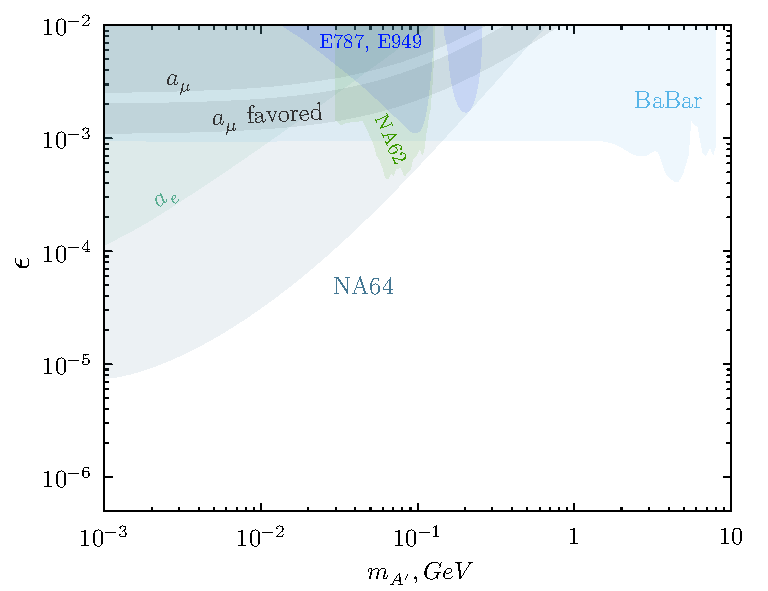
\includegraphics[width=0.45\textwidth,height=0.515\textwidth]{\pdirfour/exclusionInvisible.pdf}
  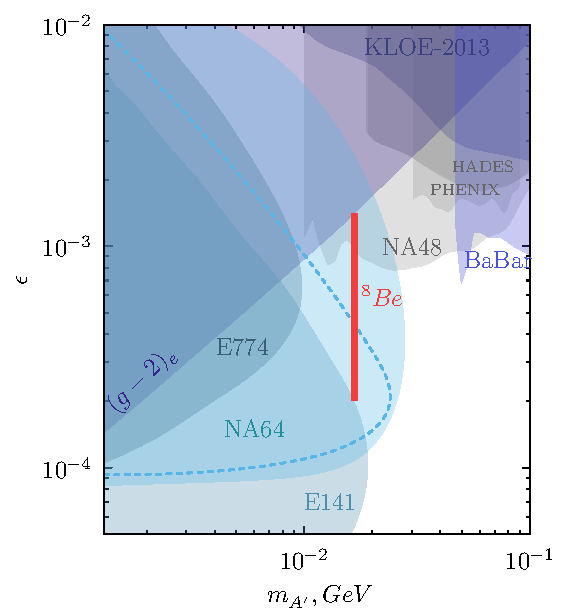
\includegraphics[width=0.45\textwidth,height=0.5\textwidth]{\pdirfour/exclusionVisible.pdf}
  \caption[Exclusion limits in the $\dmplane$]{The NA64 90\% exclusion region in the $\dmplane$ plane. The exclusion is shown for the data collected in the invisible mode setup (right) and visible mode setup (left), assuming the dominant decay is either invisible or visible respectively\cite{NA64:2019imj,Banerjee:2019hmi}. For the invisible mode, constraints from E787 and E949 \cite{PhysRevD.89.095006,Essig:2013vha},BABAR \cite{PhysRevLett.119.131804}, and recent NA62 results \cite{CortinaGil:2019nuo} are also shown, together with the muon $a_{\mu}$ favored area. For the visible mode, constraints from the experiments E774 \cite{PhysRevLett.67.2942}, E141 \cite{PhysRevLett.59.755}, BABAR \cite{babar1}, KLOE \cite{kloe2}, HADES \cite{hades}, PHENIX \cite{phenix}, NA48 \cite{na48} and bounds from the anomalous magnetic moment of the electron \cite{PhysRevD.89.095006} are shown. A blue dotted line shows the previous limit obtained with the analysis of the 2017 data. A thick red line shows the full parameter space that explains the $\DMX$-anomaly with the existence of a new protophobic vector boson \cite{PhysRevD.95.035017}, $2 \times 10^{4} < \epsilon< 1.4 \times 10^{-3}$. Currently, NA64 exclude coupling $\epsilon < 6.8 \times 10^{-4}$ for a $\DMX$ mass of 16.7 \mev.}
  \label{fig:exclusion-dmplane}
\end{figure}

\begin{figure}[bth!]
  \centering
  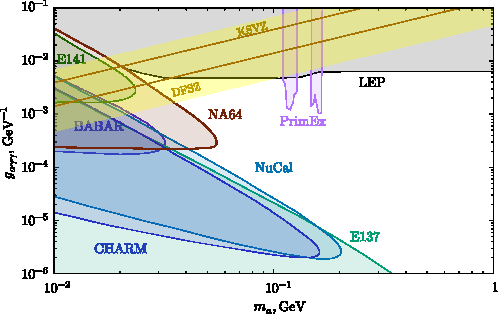
\includegraphics[width=0.7\textwidth]{\pdirfour/alps_new.pdf}
  \caption[Exclusion limits in the $(m_{a};g_{a \gamma \gamma})$ plane for ALPS and light scalar]{The 90\% exclusion limit for ALPS and light scalar particle obtained from the full dataset 2016-2018 in NA64 plotted in the $(m_{a};g_{a \gamma \gamma})$ plane. The yellow band represents the parameter space for the benchmark DFSZ \cite{DINE1981199} and KVSZ \cite{PhysRevLett.43.103} models. Constraint from BABAR \cite{Dolan:2017osp}, E137 \cite{e137}, E141 \cite{blum}, LEP , and PrimEx \cite{PhysRevLett.123.071801} experiments, as well as limits from CHARM \cite{BERGSMA1985458} and NuCal \cite{Dobrich:2019dxc} are also shown.}
  \label{fig:exclusion-dmplane-alps}
\end{figure}

\newpage

\FloatBarrier
\section{Exclusion limits in the $\dmyplane$ plane}
\label{ch4:sec:exclusion-limits-y}

The results of the invisible mode can also be interpreted in the broader framework of cosmological Dark Matter. As detailed in chapter \ref{chapter1}, various Dark Sector models motivate sub-$\gev$ scalar and Majorana or pseudo-Dirac fermion Dark Matter coupled to Dark Photons \cite{battaglieri2017cosmic}. We use the requirement of the thermal freeze out of DM annihilation into SM to derive a relation between the interesting parameters of the model \cite{na64-prd}:

\begin{equation}
  \label{eq:ad-freeze-out}
  \alpha_D \simeq 0.02 f\left(\frac{10^-3}{\epsilon}\right)^2\left(\frac{m_{\DM}}{100 \mev}\right)^2\left(\frac{10 \mev}{m_{\chi}}\right)^2
\end{equation}

Where we define $\alpha_d = e^2_D/4\pi$, $f\lesssim 10$ for a scalar \cite{deNiverville:2011it}, and $f\lesssim 1$ for a fermion \cite{PhysRevD.91.094026}. Dark Matter models can be classified by the spin and masses of the mediator. Here we consider the vector case that is relevant to us, and we remind that scalar mediators are restricted by the non-observation of rare B-meson decay \cite{battaglieri2017cosmic}. Hence, we cast our results in the $\dmyplane$ plane using Eq.\ref{eq:dmplane-y-dp} after setting values for $\alpha_D$ and $m_{\chi}$. In Fig.\ref{fig:dm-alpha-excl} the models excluded are presented, assuming $m_{\DM} = 3m_{\chi}$ and taking $\alpha_D=0.1$ and $\alpha=0.5$ as benchmark values for comparison. Those values are compatible with the derivation of running coupling in the dark sector of \cite{Davoudiasl:2015hxa}, which argues an upper limit on $\alpha_D$ to allow perturbative calculations. We used $f=0.25$ for the case of pseudo-Dirac fermion and $f=3$ for the case of Majorana. It should also be noted that for the case of smaller $\alpha_D$ the experimental bound shown would be more restrictive, as the yield in NA64 depends on just $\epsilon^2$ and not $\epsilon^4 \alpha_D$ like classical beam-dump searches. In conclusion, while the results are promising, the region compatible with the observed relic density under the assumption of a freeze-out mechanism is still not in the NA64 experimental sensitivity. A larger number of EOT needs to be collected to probe that region of parameter space. This topic will be further explored in chapter \ref{chapter5}.

\begin{figure}[bth!]
  \centering
  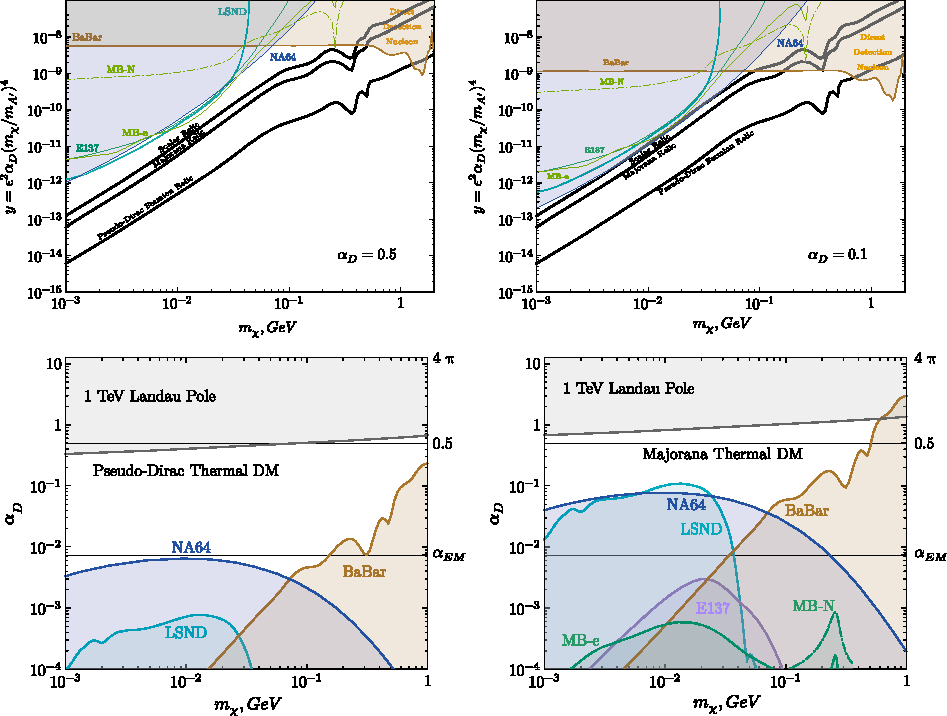
\includegraphics[width=\textwidth]{\pdirfour/tldra-complete.pdf}
  \caption[Exclusion limit in the $dmyplane$ for scalar, pseudo-Dirac and Majorana type of light Dark Matter]{The top rows show the NA64 limits in the $\dmyplane$ plane obtained for $\alpha_D = 0.5$ (left panel) and $\alpha_D = 0.1$ (right panel) from the full 2016-2018 data set. The bottom rows shows the same constraint in the $\dmaplane$ for the pseudo-Dirac (left panel) and Majorana (right panel) Dark matter. The limits are shown in comparison with the bounds obtained from the results of the LNSD \cite{deNiverville:2011it}, E137 \cite{e137}, MiniBooNE \cite{Aguilar-Arevalo:2018wea}, BABAR \cite{babar1} and direct detection experiments \cite{Essig:2012yx}. The favored parameters to account for the observed relic DM density for the scalar, pseudo-Dirac and Majorana type of light DM are shown as the lowest solid line in top plots \cite{Berlin:2018bsc}.}
  \label{fig:dm-alpha-excl}
\end{figure}

%%% Local Variables:
%%% mode: latex
%%% TeX-master: "../PhDthesis"
%%% End: